
We will perform two suites of simulations; one will be a pair of high resolution $2048^3$
simulations of plasma turbulence, and the other will be three high resolution
AMR simulations of isolated galaxies.  There will be many things to measure from
these simulations, our first focus is to study the observed polarization produced by
plasma turbulence in the galaxy.  The study of this dusty, magnetized turbulence
will allow us to remove the polarization signal due to our own galaxy from the
polarization of the cosmic microwave background (CMB).  This, in turn, will
allow us to see gravitational waves from the big bang.

The code we will use is Enzo \citep{Collins10, Bryan14}.  This is an open source
adaptive mesh refinement (AMR) code that has been used for many astrophysical
applications on the world's largest computers.  Enzo uses higher order Godunov
methods to solve the MHD equations, fourier transform based methods for gravity,
and the algorithm of \citet{Berger89} for the AMR.  The code also includes
chemistry and star particles, but their cost is negligible compared to the MHD,
Gravity, and AMR.  Here we will profile the performance of the three primary
systems in the manner they will be used in the proposed simulations.

The cost of each of the three systems is independent of the state of the plasma,
so we simulate boxes with uniform density and temperature for simplicity.  We
perform three suites of study.  For the MHD and Gravity study, single resolution
boxes are used.  For the AMR study, we use the same constant work-per-level
that will be employed in our galaxy simulations; the central 1/8th of the box is
refined by a factor of 2.  
While the proposed simulations will use 8 levels of
refinement, one level is used for the scaling study.  This is enough to engage the AMR machinery that keeps the
information consistent between levels, without the expense of a full AMR
timestep.  For 8 levels, 512 steps are taken across all levels, which is not
necessary to measure performance and scaling.
We have additionally tested the full 8 level configuration at scale, and it
performs exactly as expected from the scaling.

We estimate the cost for our simulations as 
\begin{align}
SU &= t_{wall} N_N\\
t_{wall} &= \frac{\sum_\ell N_Z N_U}{\zeta}\frac{1}{N_C},
\end{align}
where $N_N$ is the number of nodes, $N_Z$ is the number of zones per level,
$N_U$ is the number of updates per level, $N_C$ is the number of cores, and most
importantly $\zeta$ is the cost in (zone-updates)/(core-second.)  Given perfect
scaling, $\zeta$ is independent of the number of cores.  We model the actual
performance by measuring $\zeta$ as we increase $N_Z$.  By targeting the same
configuration we will use for the production simulations, this is an accurate
estimate of the ultimate cost.

The result of the scaling study can be found in Figure \ref{fig}, which shows
the performance, $\zeta$, vs. number of cores, $N_C$.  For each simulation, we
take one root grid timestep, which includes the AMR steps in the AMR suite, then
divide by the time.  Here we
perform simulations with fixed work of $64^3$ zones per core, in three suites of
simulations.  The AMR suite has two grids of $64^3$ per core.  We use $256, 512,
1024, 1536,$ and $2048$ zones per side for all three suites, with the AMR suite
including a second level of the same number of zones.  We use 56 cores per node
throughout.  As the number of cores is not an exact multiple of 56, one node has
a few idle cores, but this is not enough to impact the scaling.  


\begin{table}[h]
\begin{center}
\caption{The number of nodes, $N_N$, zones, $N_Z$, and cores, $N_C$ used for each
node in our scaling study.}
\label{table1}                                                                                                                                                               
\begin{tabular}{rrr}
$N_N$ & $N_Z$ & $N_C$\\
\hline
2 & $256^3$ & $64$\\
10 & $512^3$ & 512 \\
74 & $1024^3$ & 4096 \\
274 & $1536^3$ & 13,824\\
586 & $2048^3$ & 32,768\\
\hline
\end{tabular}                                                                                                                                                               
\end{center}
\end{table}                                                                                                                                                                

\begin{figure} \begin{center}
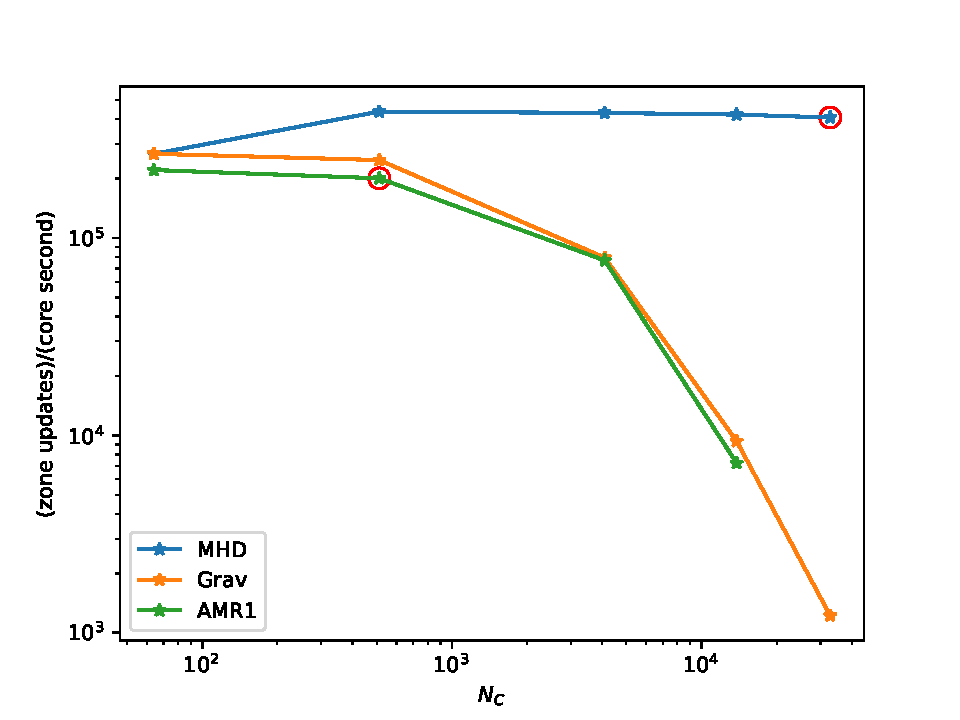
\includegraphics[width=\textwidth]{g57_zoneup.pdf}
\caption[ ]{The performance, $\zeta$ vs. number of cores, $N_C$,  for Enzo in
three configurations.  The MHD solver alone (blue curve) scales quite well.  The
orange curve shows MHD and the gravity solver, while the green curve shows the
MHD solver, gravity solver, and AMR overhead. Red circles show the target
simulation configuration.}
\label{fig} \end{center} \end{figure}

The blue curve in Figure \ref{fig} shows the scaling of the MHD solver.  This
component scales with the number of zones simply as $N_Z$, so as we increase
both in concert we see very little drop in performance.
 $\zeta$=4.4\sci{5} for 10 nodes, and $\zeta=4.1\sci{5}$ for 586 nodes, less
than 10\% decrease in performance for a factor of 64 in core count.  It is this
outstanding scaling that enables us to perform such large simulations.

The orange curve in Figure \ref{fig} employs the MHD solver and the gravity
solver.  The cost of the FFT based gravity sovler increases as $N_Z \ln N_Z$, so the
performance, $\zeta$, suffers from the increased cost.  Additionally, the FFT is
done on pencils spaning the domain, but the data is stored in cubes.  This
rearangement of data also costs in the scaling.  

The AMR suite can be seen in the green curve in Figure \ref{fig}.  This suite
employs the MHD solver, gravity solver, and AMR overhead, which represents the
performance of the galaxy simulations.  The additional cost above the gravity can be
seen to be small on all runs.  
We were not able to run $2048^3$ with one level of
additional $2048^3$ due to a memory problem.
This is quite far from our current goals, so not solved at this time; we believe
that this is a minor bug, and will be solved when we are ready for that scale.

The red circles show $\zeta$ for the proposed simulations.  The turbulence
simulations will run $2048^3$ zones on 586 nodes, with a performance of
$\zeta=4\sci{5}$.  
The AMR simulations will use 8 levels of roughly $512^3$ per level on 10 nodes,
with a performance of $\zeta=2\sci{5}$.  





